\documentclass{beamer}

\usepackage{fontspec}
\usepackage[ngerman]{babel}
\usepackage{verbatim}
\usepackage{fancyvrb}
\usepackage{listings}
\usepackage{csquotes}
\usepackage{pst-electricfield}

\usepackage{tikz}
% Vector Styles
\tikzset{
  load/.style   = {ultra thick,-latex},
  stress/.style = {-latex},
  dim/.style    = {latex-latex},
  axis/.style   = {-latex,black!55},
}

% Drawing View
\tikzset{dimetric2/.style={
  x={(0.935cm,-0.118cm)},
  y={(0.354cm, 0.312cm)},
  z={(0.000cm, 0.943cm)},
}}

\usepackage{biblatex}
\addbibresource{bib.bib}

\usetheme{Berlin}
\usecolortheme{beaver}

\usefonttheme{professionalfonts} % using non standard fonts for beamer
\usefonttheme{serif} % default family is serif
\setmainfont{Liberation Serif}


\lstset{
    basicstyle=\ttfamily,
    language=[LaTeX]TeX,
    % Other customizations...
}



\title{Einf\"uhrung in \LaTeX}
\author{Daniel Renschler}
\date{17. Juli 2023}


\begin{document}


\begin{frame}
    \titlepage 
\end{frame}


\begin{frame}
    \tableofcontents
\end{frame}


\section{\LaTeX?}
\begin{frame}{Was ist \LaTeX?}


    \begin{itemize}
        \item Knuth hat \TeX gemacht
        \item Lamport hat dann \LaTeX daraus gemacht
    \end{itemize}

    \begin{columns}
        \column{0.5\textwidth}
        
        \hfill
        \column{0.4\textwidth}
        \begin{figure}[htpb]
            \centering
            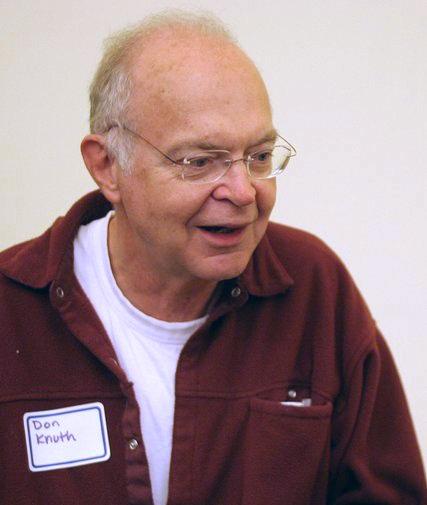
\includegraphics[width=0.7\textwidth]{./figs/tex-knuth.jpg}
            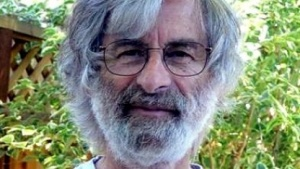
\includegraphics[width=0.7\textwidth]{./figs/latex-lamport.jpg}
        \end{figure}
    \end{columns}

\end{frame}



\begin{frame}{Warum \LaTeX?}
    \begin{itemize}
        \item Ist sehr intuitiv.
        \item Unendlich extensiv mit packages.
        \item K\"ummert sich um viel von alleine
        \item Man muss sich nicht mit Typografie und Vergleichbarem vertraut machen\footnote{Es funktioniert einfach und sieht gut aus.}.
        \item Macht spa\ss
    \end{itemize}
\end{frame}



\begin{frame}{Warum nicht Word? (oder andere WYSIWYG\footnote{WYSIWYG = What you see is what you get} software)}
    \begin{itemize}
        \item Word macht es schwerer \"Anderungen an gro\ss{}en Dokumenten vorzunehmen.
        \item Bibliografien werden nicht automatisch gemacht, auch Zitierstil nachtr\"aglich \"anderbar.
        \item Seitenzahlen, Referenzen, etc. werden nicht automatisch erzeugt.
        \item \textit{kann man nicht in Vim benutzen.}
    \end{itemize}
    
\end{frame}




\begin{frame}{Nutzzwecke}

    \begin{itemize}
        \item Ausarbeitungen/Laborberichte
        \item Pr\"asentationen
        \item Dokumente
        \item Lebenslauf
        \item B\"ucher
    \end{itemize}
\end{frame}




\section{Beispiele}
\begin{frame}{Berichte}
    \begin{itemize}
        \item Laborberichte 
    \end{itemize}
    \begin{figure}[htpb]
        \centering
        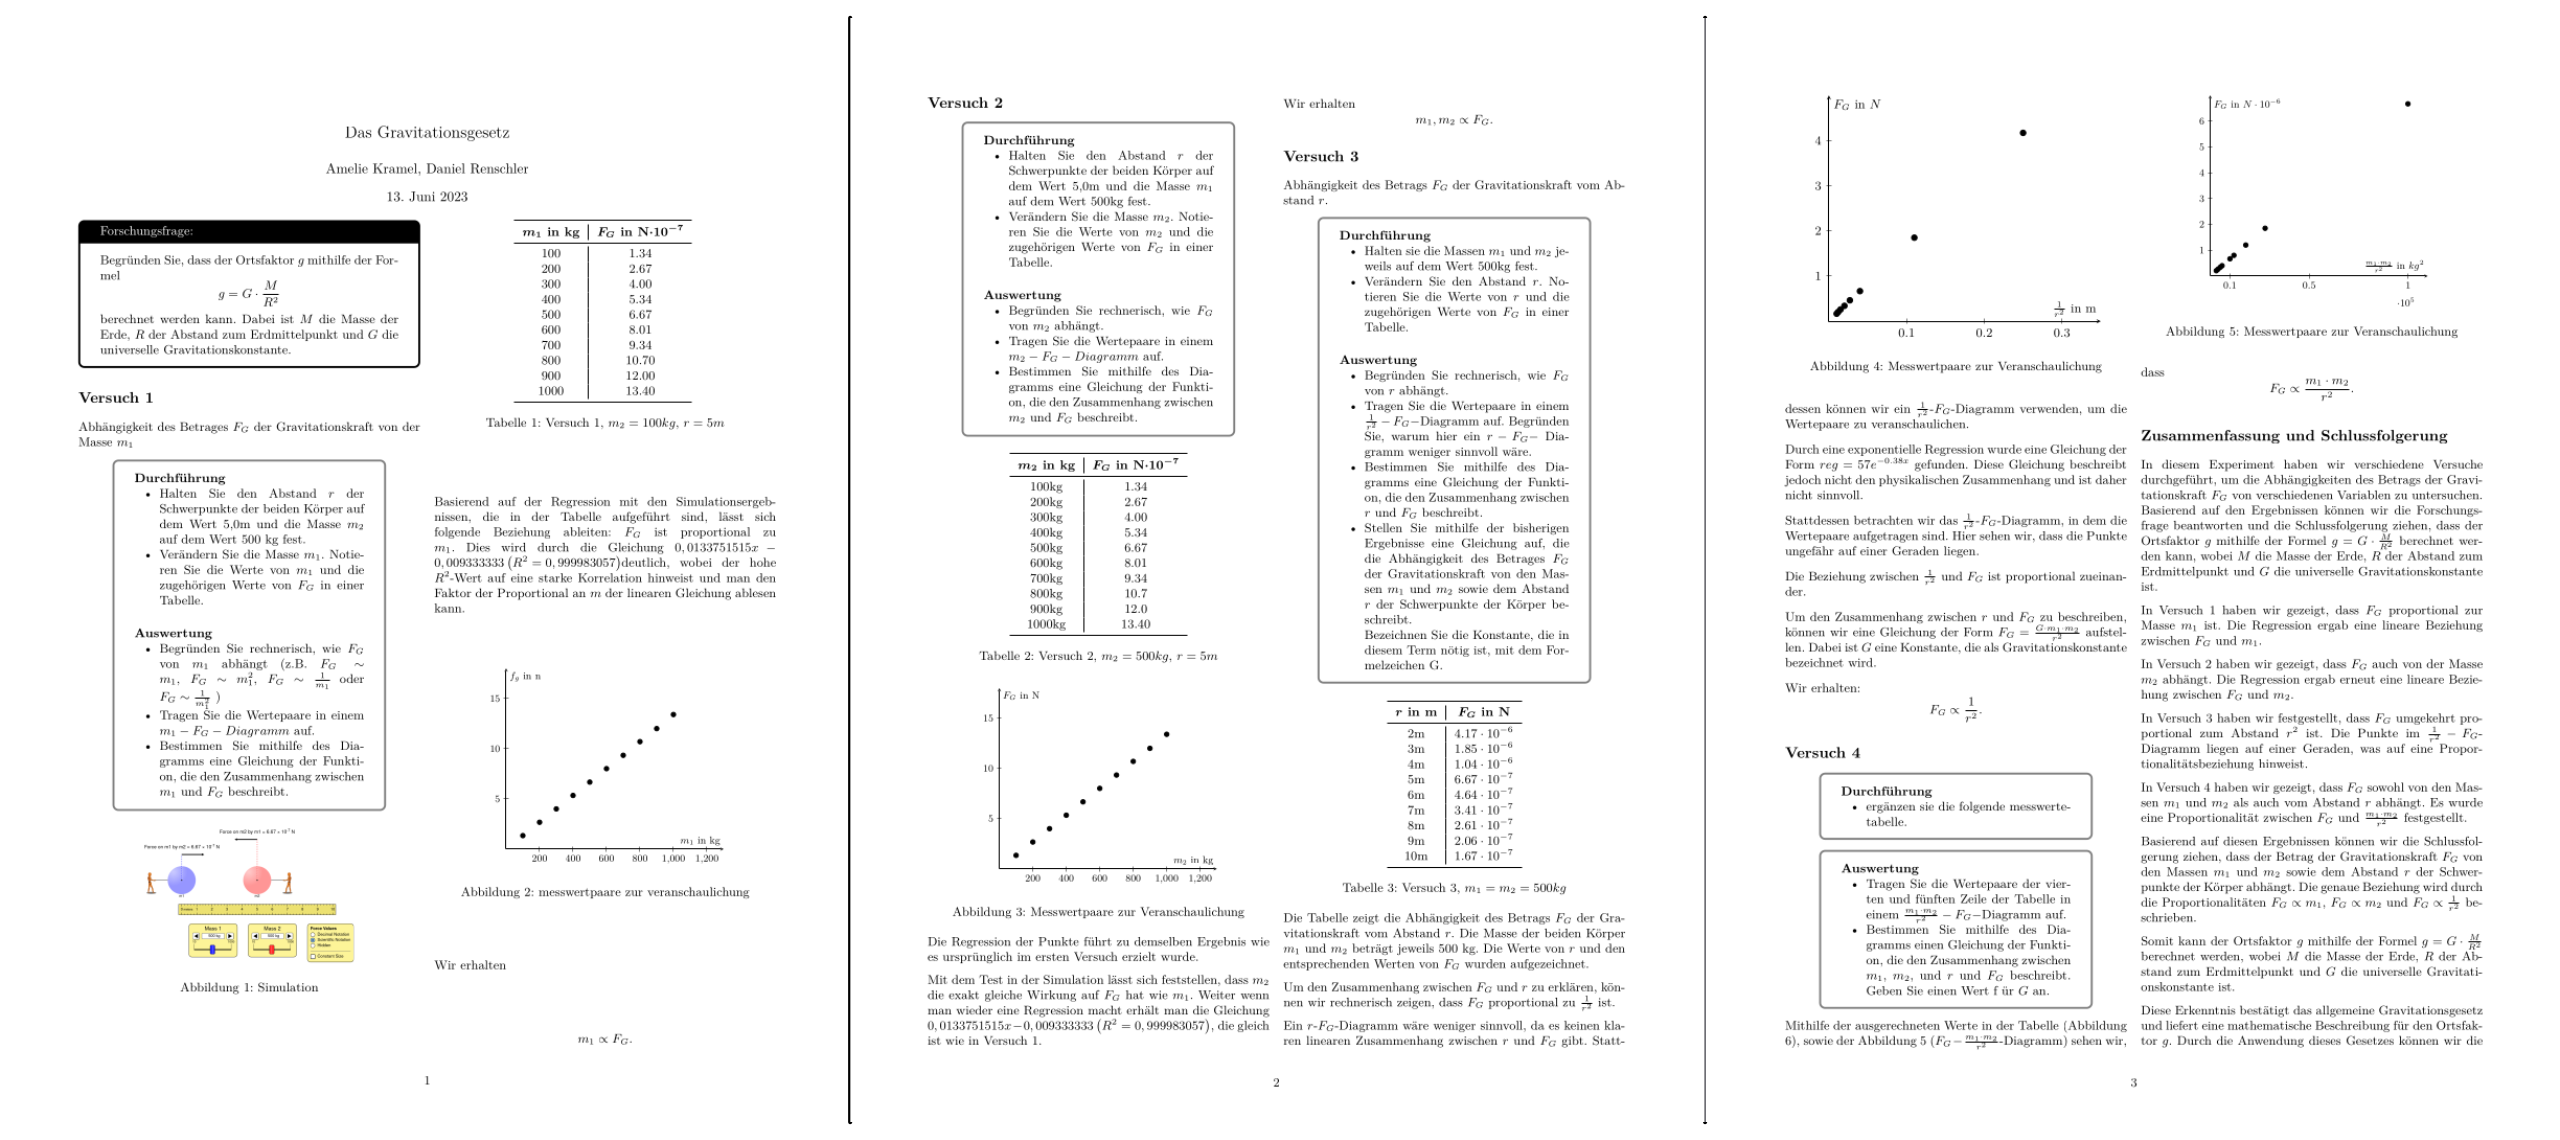
\includegraphics[width=1\textwidth]{./figs/am stueck.png}
        \caption{Laborprotokoll Gravitationsgesetz}
        \label{fig:}
    \end{figure}
\end{frame}



\begin{frame}{Paper}
    \begin{figure}[htpb]
        \centering
        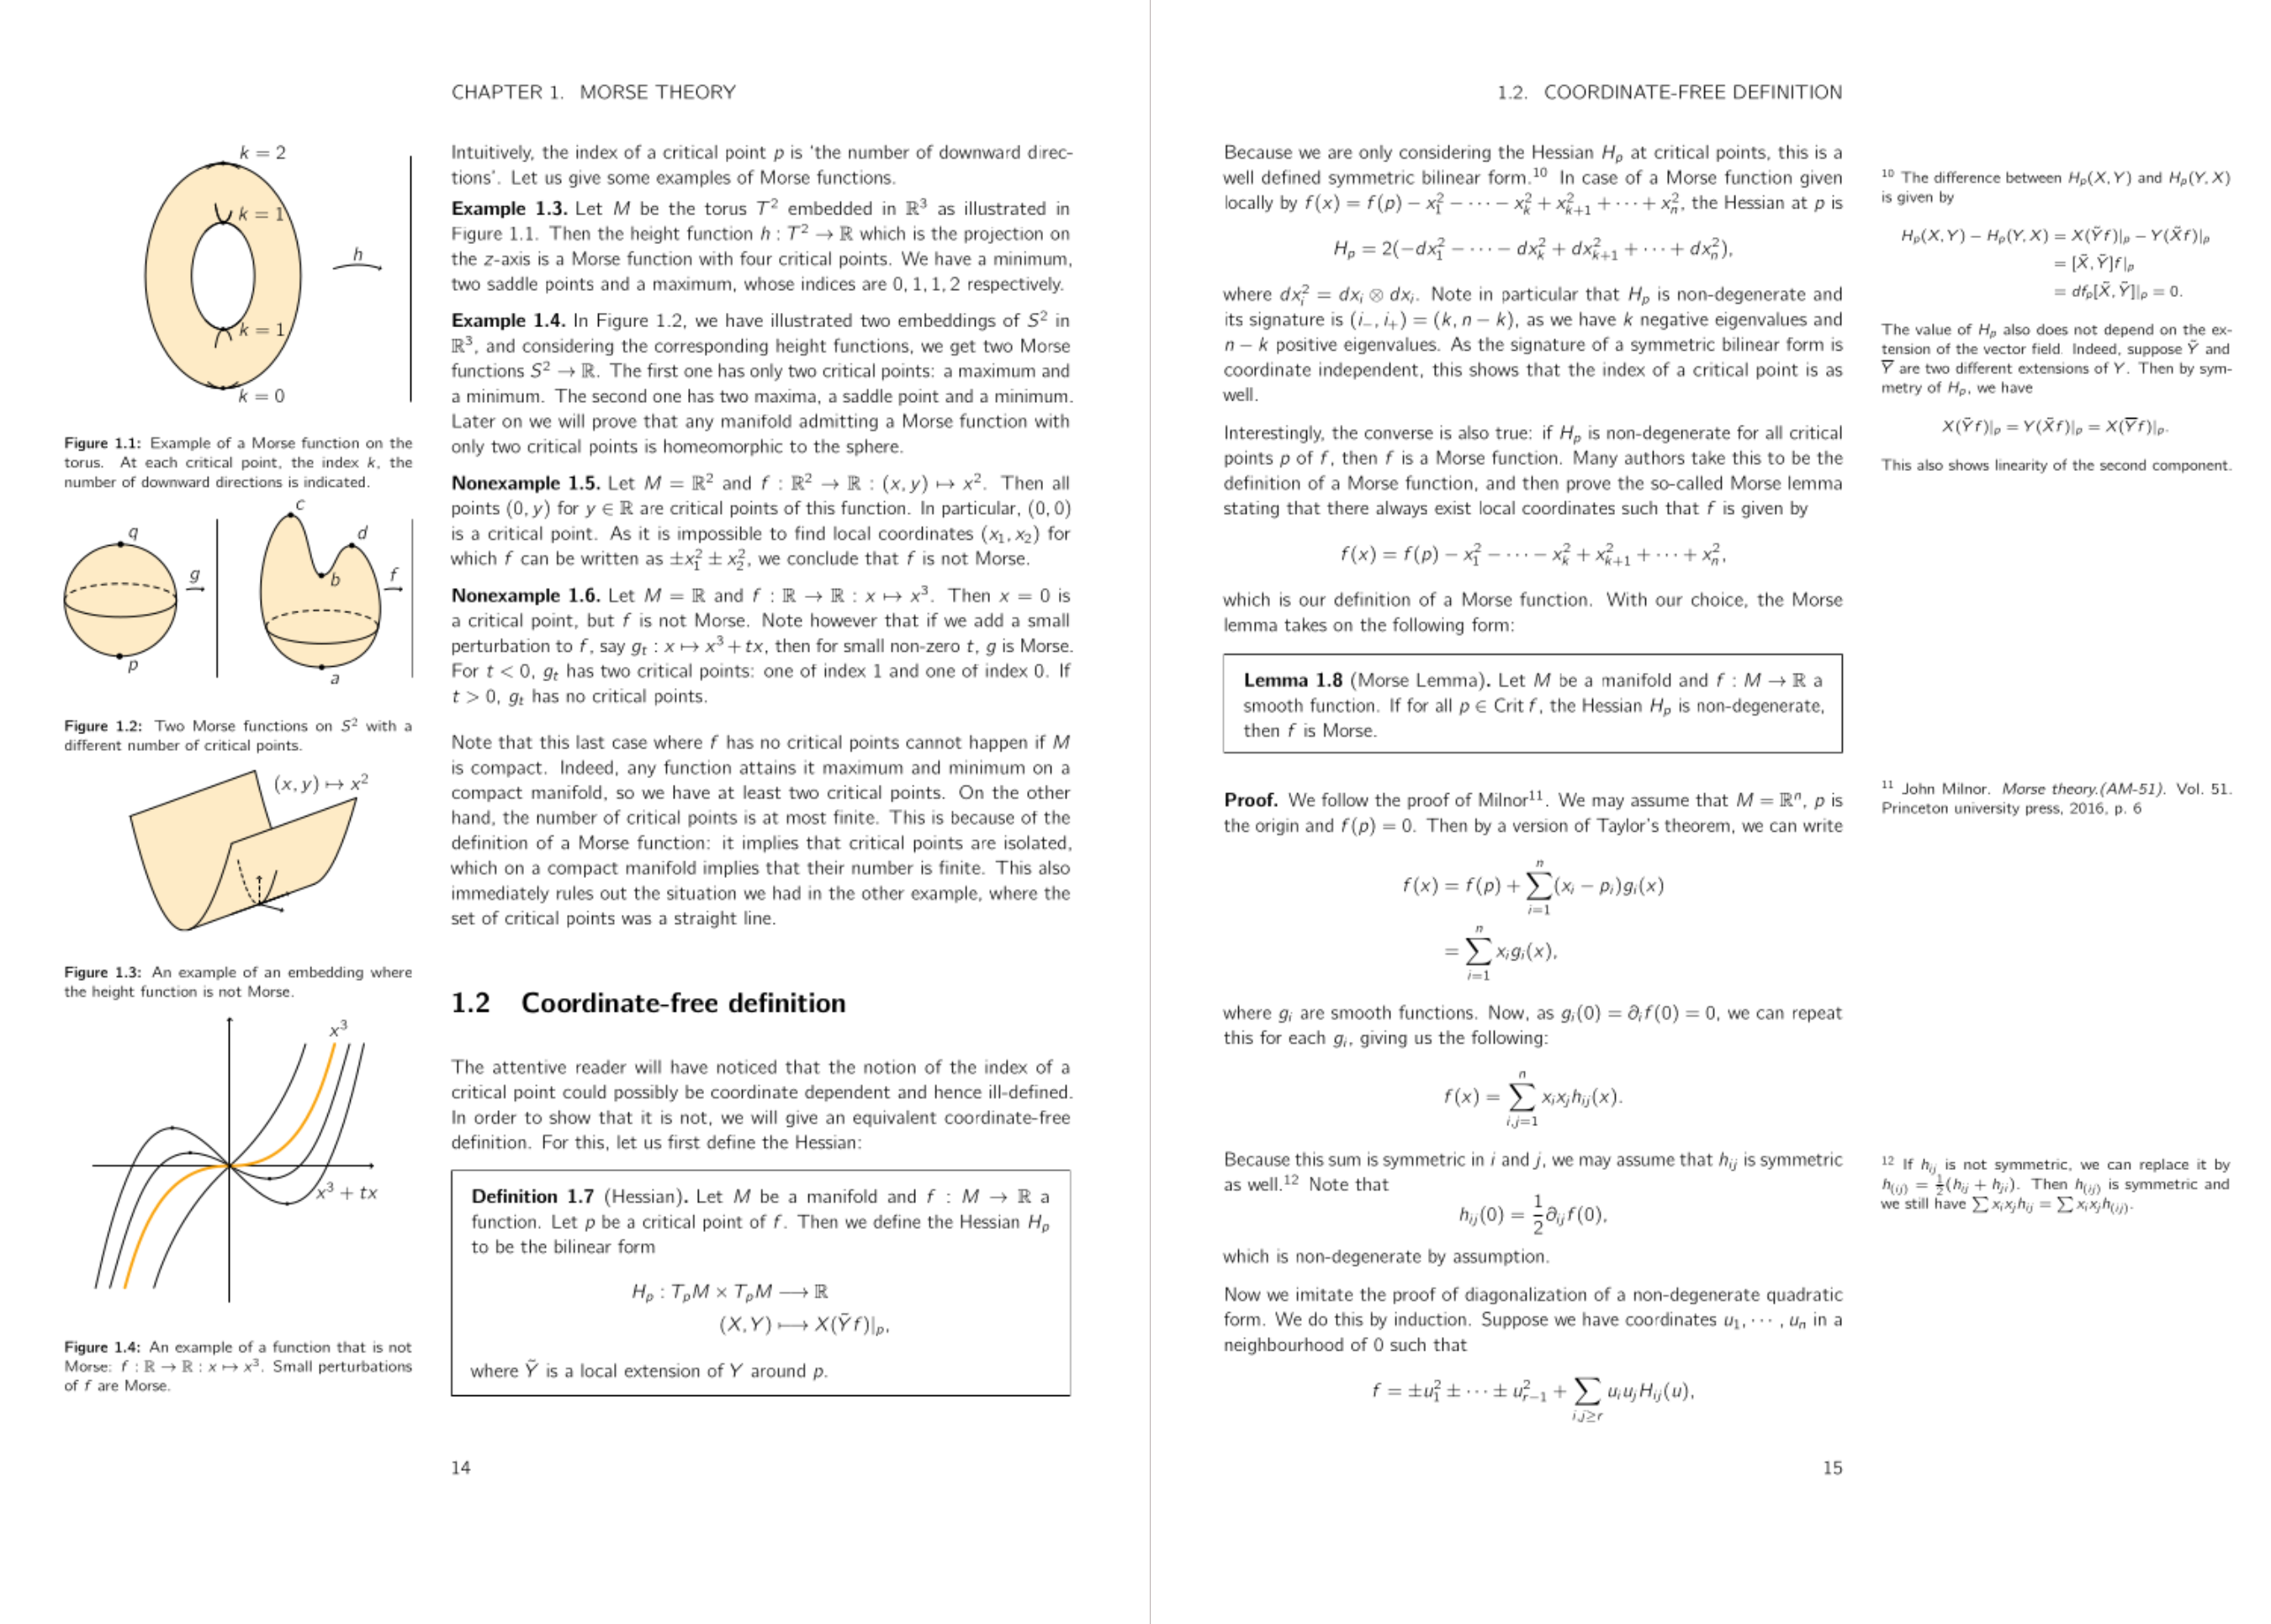
\includegraphics[width=0.7\textwidth]{./figs/example-paper.png}
        \caption{Auszug einer Masterarbeit \"uber Morse Theory}
    \end{figure}
\end{frame}


\begin{frame}{Beispiel 1}


Beispiele:
\begin{itemize}
    \item Irgendwas mit Euler \cite{baranek2023randomized}
        \[ \mathcal{L} = \frac{\partial}{\partial t}+ \frac{1}{2}\sum_{k=1}^{m}\frac{\partial^2}{\partial y_{k}^2} .\] 
\end{itemize}


\begin{itemize}
    \item Analysis Aufgabe: 
        \[ \lim_{x\to \int_0^{\infty} \sqrt{t}e^{-t}dt}\left( \left( \sum_{n=0}^{\infty}\frac{x^{4n_4}}{(2n+1)(4n+3)(4n+4)} \right)''  \right) .\] 
\end{itemize}
\end{frame}

    



\begin{frame}{Toeplitz Matrix}
    \[ A=\begin{bmatrix}
            a_0 & a_{-1} & a_{-2} & \ldots & \ldots  &a_{-n+1}  \\
            a_1 & a_0  & a_{-1} &  \ddots   &  &  \vdots \\
            a_2 & a_1 & \ddots  & \ddots & \ddots& \vdots \\ 
            \vdots &  \ddots & \ddots &   \ddots  & a_{-1} & a_{-2}\\
            \vdots &         & \ddots & a_1 & a_0 &  a_{-1} \\
            a_{n-1} &  \ldots & \ldots & a_2 & a_1 & a_0
        \end{bmatrix} .\] 
\end{frame}



\begin{frame}{Physik Beispiel}
    Sequential Quantum Circuits as Maps between Gapped Phases.\cite{chen2023sequential}
    \begin{align*}
        \frac{1}{|G|}\sum_g X^g_i &\to \sum_h T^h_{i-1}T^h_i, \quad i=2,\ldots,N,  \\
        \frac{1}{|G|} \sum_g X_1^g &\to \frac{1}{|G|} \sum_{h,h'}e^{-\frac{2\pi i}{|G|}(h'-h)g}T_1^hT^{h'}_N \prod^N_{i=1}X_i^g,  \\
        \sum_h T^h_i T^h_{i+1} &\to \frac{1}{|G|} \sum_g X_i^g, i=2,\ldots,N  \\
        \sum_h T^h_1 T^h_2 &\to \frac{1}{|G|} \sum_g X_1^g \prod_{i=1}^N X_i^g.
    \end{align*}
\end{frame}


\begin{frame}{Abbildungen}


    \begin{tikzpicture}
        \node (origin) at (0,0) {}; % shift relative baseline
        \coordinate (O) at (2,3);
        \draw[fill=gray!10] (O) circle (1);
        \draw[fill=white] (O) circle (0.75) node[below,yshift=-1.125cm] {Signpost Cross Section};
        \draw[dim] (O) ++(-0.75,0) -- ++(1.5,0) node[midway,above] {$d_i$};
        \draw[dim] (O) ++(-1,1.25) -- ++(2,0) node[midway,above] {$d_o$}; 
        \foreach \x in {-1,1} {
            \draw (O) ++(\x,0.25) -- ++(0,1.25);
        }
    \end{tikzpicture}
    \begin{tikzpicture}[dimetric2, scale=0.7]
        \coordinate (O) at (0,0,0);
        \draw[axis] (O) -- ++(6,0,0) node[right] {$x$};
        \draw[axis] (O) -- ++(0,6,0) node[above right] {$y$};
        \draw[axis] (O) -- ++(0,0,6) node[above] {$z$};
        \draw[fill=gray!50] (0,0,-0.5) circle (0.5); 
        \fill[fill=gray!50] (-0.46,-0.2,-0.5) -- (0.46,0.2,-0.5) -- (0.46,0.2,0) -- (-0.46,-0.2,0) -- cycle;
        \draw[fill=gray!20] (O) circle (0.5);
        \draw (0.46,0.2,-0.5) -- ++(0,0,0.5) node[below right,pos=0.0] {Fixed Support};
        \draw (-0.46,-0.2,-0.5) -- ++(0,0,0.5);
        \draw[fill=gray!10] (O) circle (0.2);
        \fill[fill=gray!10] (-0.175,-0.1,0) -- (0.175,0.1,0) -- ++(0,0,4) -- (-0.175,-0.1,4) -- cycle;
        \draw (-0.175,-0.1,0) -- ++(0,0,4);
        \draw (0.175,0.1,0) -- ++(0,0,4) node[right,midway] {Steel Post};
        \draw (4,0,3.95) -- ++(0,0,-1);
        \foreach \z in {0.5,0.75,...,5} {
            \draw[-latex] (-2*\z/5-0.2,0,\z) -- (-0.2,0,\z);
        }
        \draw[load] (0,0,4) -- ++(0,0,-1.25) node[right,xshift=0.1cm] {$F_{z1}$};
        \draw[fill=gray!20] (-0.25,-0.25,5) -- (4,-0.25,5) -- (4,+0.25,5) -- (-0.25,+0.25,5) -- cycle; 
        \draw[fill=gray!50] (+4.00,-0.25,4) -- (4,+0.25,4) -- (4,+0.25,5) -- (+4.00,-0.25,5) -- cycle; 
        \draw[fill=gray!10] (-0.25,-0.25,4) -- (4,-0.25,4) -- (4,-0.25,5) -- (-0.25,-0.25,5) -- cycle; 
        \draw (4.05,0,4) -- ++(1,0,0);
        \draw (4.05,0,5) -- ++(1,0,0);
        \draw[dim] (4.5,0,0) -- ++(0,0,4) node[midway,right] {$h_1$};
        \draw[dim] (4.5,0,4) -- ++(0,0,1) node[midway,right] {$h_2$};
        \draw[dim] (0,0,3.4) -- ++(4,0,0) node[midway,below] {$b_2$};
        \coordinate (P) at (2,-0.25,4.5);
        \draw (P) -- ++(0,0,0.25);
        \draw (P) -- ++(0.25,0,0);
        \draw[dim] (2.125,-0.25,4.5) -- ++(0,0,-0.5) node[midway,right] {$z_1$};
        \draw[dim] (2,-0.25,4.625) -- ++(-2,0,0) node[midway,below] {$x_1$};
        \draw[load] (2,-2.45,4.5) -- ++(0,2.2,0) node[pos=0.0,right,xshift=0.08cm] {$F_{y1}$};
        \draw[axis,dashed,-] (O) -- (0,0,5);
        \draw (0,0,5.5) -- ++(4,0,0) node[midway,above] {$w_{z}$};
        \foreach \x in {0,0.25,...,4} {
            \draw[-latex] (\x,0,5.5) -- ++(0,0,-0.5);
        }
        \draw (-0.2,0,0) -- ++(-2,0,5) node[above,xshift=0.5cm] {$w_{x}=\frac{z}{h_1+h_2} w_0$};
    \end{tikzpicture}


\end{frame}


\section{Syntax \& etc.}
\begin{frame}{Syntax}

\begin{itemize}
    \item Commands beginnen mit \textbackslash{}, nicht zu verwechseln mit \Verb|/|
    \item Umgebungen (environments) beginnen und enden immmer gleich, man kann/muss nesten.
\end{itemize}


\end{frame}



\begin{frame}[fragile]
    \frametitle{Struktur}
Struktur die in jedem Dokument eingehalten werden muss:
    
\begin{lstlisting}
\documentclass{article}
\usepackage{tikz} % Fuer Zeichnungen
\usepackage{amsmath} % Fuer mathematische Symbole

\begin{document}
    
\end{document}
\end{lstlisting}

\end{frame}



\begin{frame}{Documentclasses}
   Gibt viele, die wichtigsten sind: 
   \begin{itemize}
        \item \Verb|article|: ``normale Klasse'' Titel ist auf erster Seite
        \item \Verb|report|:  Titel hat eigene Seitenzahlen
        \item \Verb|beamer|: F\"ur Pr\"asentationen (diese z.B.)
        \item Andere sind: \Verb|book|, \Verb|letter|, etc.
   \end{itemize}
\end{frame}



\begin{frame}{Sections}
Es gibt verschiedene an Sections.

\begin{itemize}
    \item section
    \item subsection
    \item subsubsection
\end{itemize}

Diese werden dann z.B. in Inhaltsverzeichnissen angezeigt und sich untergeordnet.

\begin{itemize}
    \item Section
        \begin{itemize}
            \item subsection
                \begin{itemize}
                    \item subsubsection
                \end{itemize}
        \end{itemize}
\end{itemize}
\end{frame}




\begin{frame}[fragile]{Fu\ss{}noten und Bibliografien}

Eine Fu\ss{}note macht man:
\begin{lstlisting}
\footnote{Fußnoteninhalt}
\end{lstlisting}

Eine Zitat macht man:
\begin{lstlisting}
\cite{Zitat}
\end{lstlisting}

Eine Bibliografie macht man:
\begin{lstlisting}
\printbibliography
\end{lstlisting}

\vfill

Fu\ss{}note\footnote{Fußnoteninhalt}

Zitat \cite{smith2017}

    
\end{frame}



\section{Anderes}
\begin{frame}{Wie man es benutzt}



    \begin{itemize}
        \item Arch-basiert: \Verb|pacman -S texlive-basic|
        \item Debian-basiert: \Verb|apt-get install texlive-full|
        \item MacOS: \Verb|MiKTeX|
        \item Windows: \Verb|MacTeX|
    \end{itemize}
\end{frame}


\begin{frame}{Wie Ich es benutze}
    \begin{figure}[htpb]
        \centering
        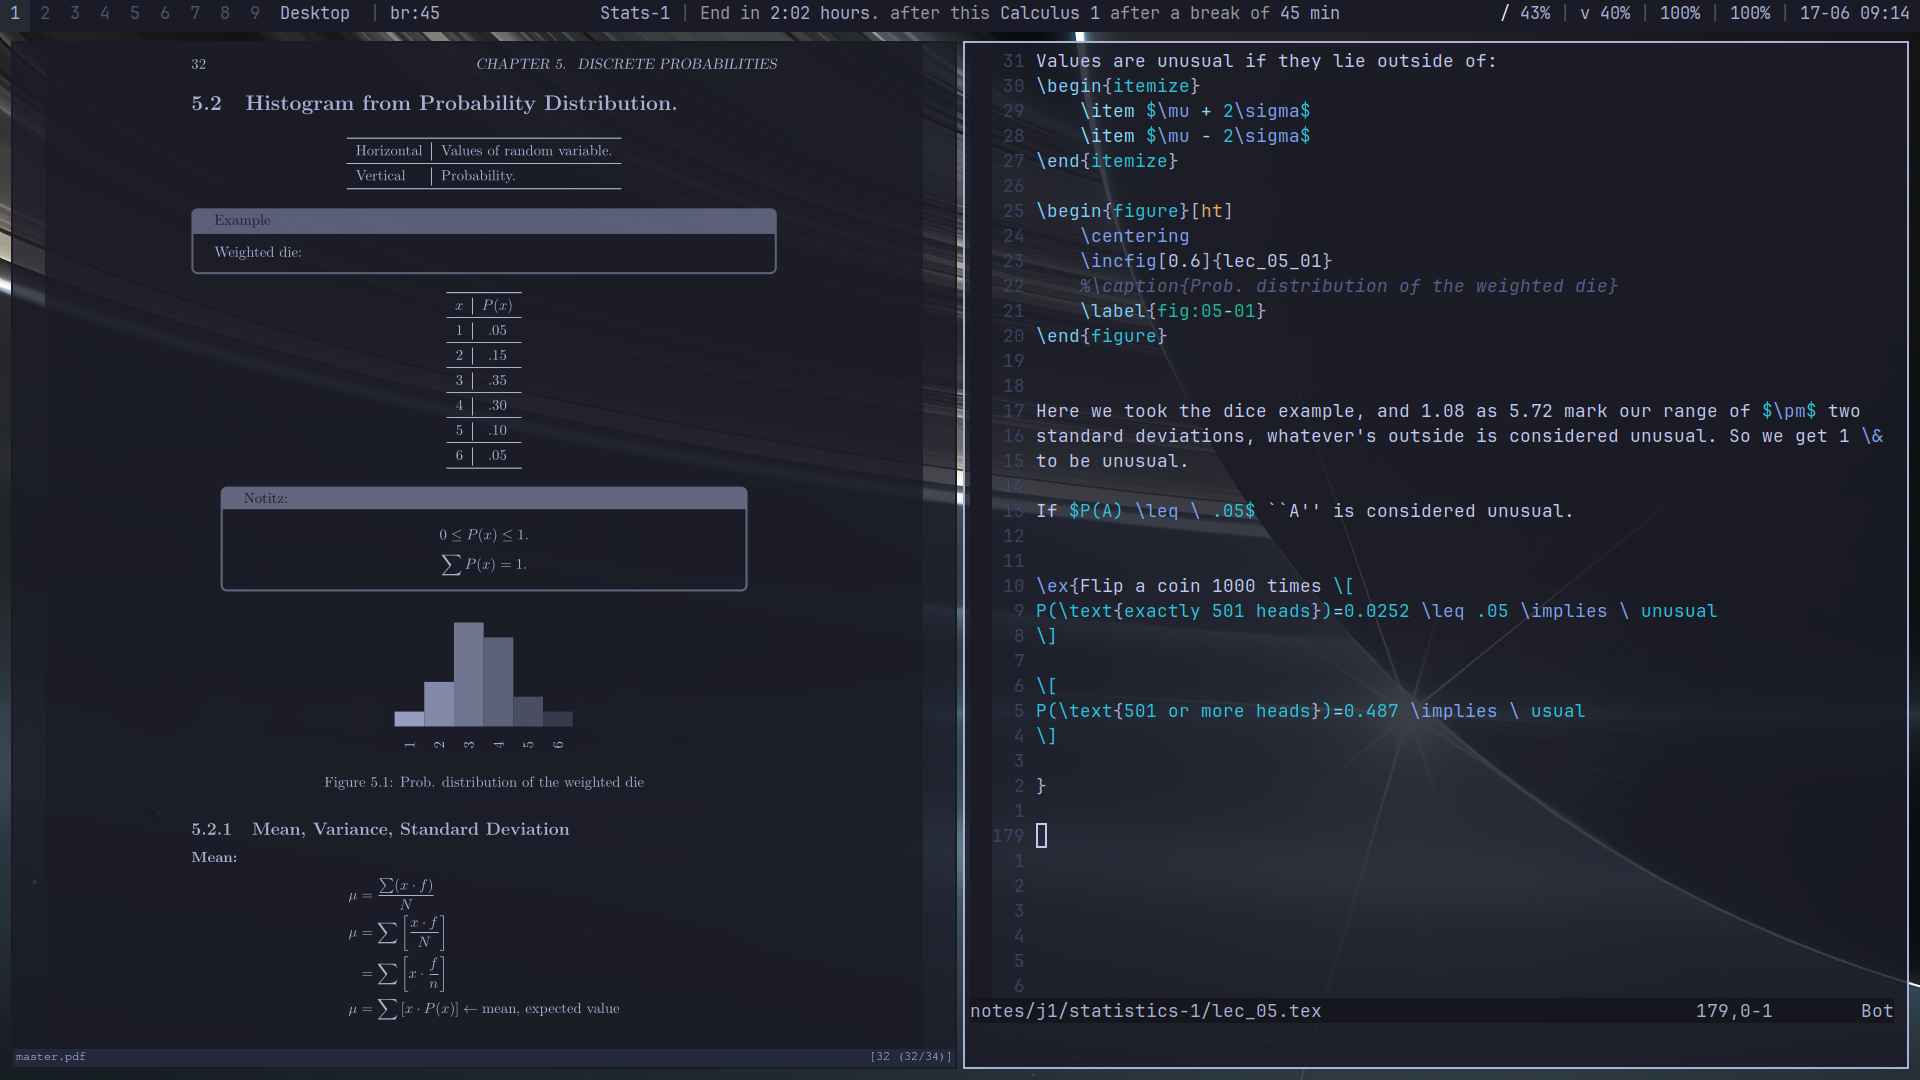
\includegraphics[width=\textwidth]{./figs/workflow.png}
        \label{fig:workflow-png}
    \end{figure}
\end{frame}


\begin{frame}{Weitere Resourcen}
    \begin{itemize}
        \item diese Pr\"asentation: \url{https://github.com/d-rens/LaTeX-Einfuehrung/}
        \item \LaTeX\ Tutorials, von Luke Smith
        \item Overleaf Tutorials
        \item ``The \TeX book", von Donald E. Knuth
    \end{itemize}
    
\end{frame}



\begin{frame}{Literatur}
    \printbibliography
    
\end{frame}





\end{document}
